\section{Analysis}

Here is the analysis. I have a made table referenced as table \ref{tab:sample_table}. Also made a figure \ref{fig:sample_figure}.

\begin{figure}[ht]
    \centering
    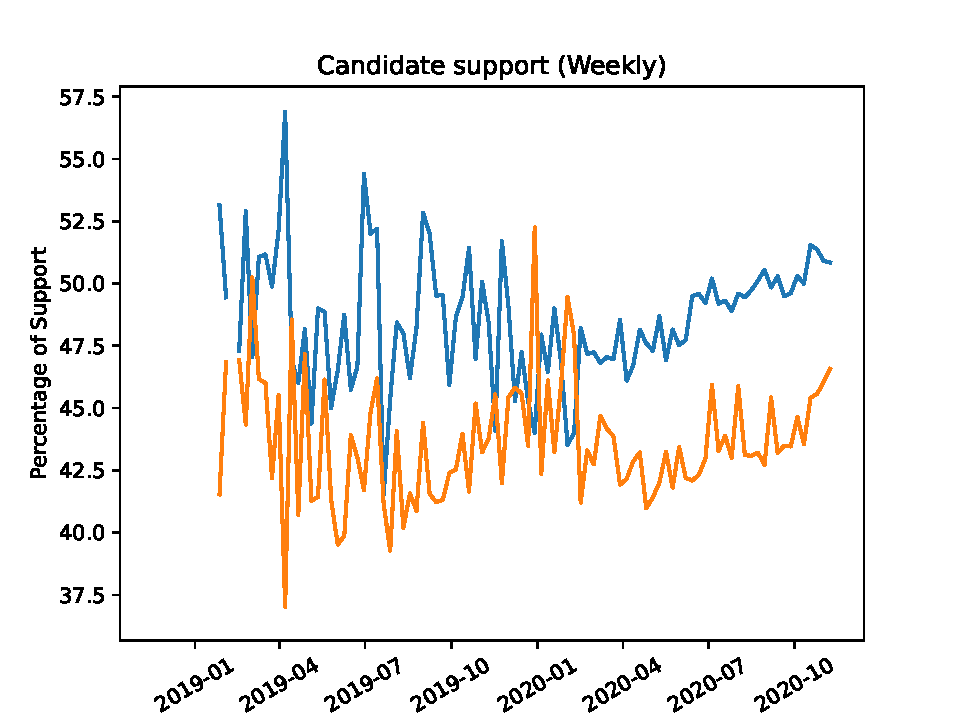
\includegraphics[width=0.8\textwidth]{../output/figures/weekly_candidate_support.pdf}
    \caption{Percentage of support for 2020 candidates of the American Election}
    \label{fig:sample_figure}
\end{figure}

\begin{table}[ht]
    \centering
    \begin{tabular}{lr}
\toprule
Candidate Name & Percentage Support \\
\midrule
Donald Trump & 44.47 \\
Joe Biden & 50.21 \\
\bottomrule
\end{tabular}

    \caption{Aggregate numbers of support}
    \label{tab:sample_table}
\end{table}

\subsection{How to make equations}

Also an example of how to make equations. Inline: $\alpha \sum x^2 = s_j$

If you want to do a standalone equation

\begin{equation}
    y = a x^2 + b x + c
\end{equation}